\chapter{\statusorange Topics}
\label{chap:topics}

\section{Introduction}

% conclusions from chapter 5:
% two motivations:
% The first one, is to find in which topics propaganda varies mostly across the political spectrum. There may be some topics where the discussion is not using a lot of propaganda techniques to drive the reader in a certain direction, or where the usage may not be very distinctive (e.g., when talking about sports, Left and Right persuasion may be quite difficult to tell apart).
% With an analysis of the topics, we can find the ones where the detected propaganda differs the most, and therefore where we can try to recognise automatically more easily the political leaning of a news article by using the propaganda features.

% % Motivation 2
% And another strong motivation to analyse the topics is to try to locate where the current approach to propaganda detection might have some issues in being accurate.
% % Find topics where propaganda detection might have some problems
% We will perform this analysis and try to find insights that could lead to the development of future propaganda detection resources (e.g., datasets) that are less subject to the imbalance problems that we found in this chapter.



% what

This new chapter introduces the last ingredient of our analysis: \emph{Topic}.
In our last chapter, we concluded with the need to analyse the topics of the articles for two main reasons:

\begin{enumerate}
    \item finding the topics where propaganda varies mostly across the political spectrum. There may be some topics where the discussion is not using a lot of propaganda techniques to drive the reader in a certain direction, or where the usage may not be very distinctive (e.g., when talking about sports, Left and Right persuasion may be quite difficult to tell apart). With an analysis of the topics, we can find the ones where the detected propaganda differs the most, and therefore where we can try to recognise automatically more easily the political leaning of a news article by using the propaganda features.
    \item analyse the topics is to try to locate where the current approach to propaganda detection might have some issues in being accurate. We will perform this analysis and try to find insights that could lead to the development of future propaganda detection resources (e.g., datasets).
\end{enumerate}


% why
Why?

% RQ

RQs:
\begin{itemize}
    \item RQ1: How can we optimise the definition of topic in order to have enough details?
    \item RQ2: How propaganda changes across topics and leanings?
    \item RQ3: knowing the topic, does it make classification (prop-->leaning) easier?
    \item RQ4: can we find some topics where propaganda detection is not working as expected? (????)
\end{itemize}

% How
How?

How this relates to other chapters


structure (similar to chap 4 and 5):
- new ingredient: topic
- combination with previous ingredients

% findings
findings


two documents:

Experiment 7: contains an analysis of different ways of extracting/using topics on my dataset. Here I show some breakdown by topic using some topics annotations in the dataset (AllSides topics), and also with the values from TextRazor (CoarseTopics, Fine-grained topics, but not yet using the hierarchical MediaTopics)

Expanding the topics of AllSides: also includes the analysis of MediaTopics (IPTC)


For the code, I have two parts:
https://github.com/MartinoMensio/textrazor-bulk-annotate which can be used to annotate a dataset.
attached the code from a private repository (bcanalytics) which contains some functions to handle the taxonomy (file src/textrazor.py ) and to plot the sunburst diagrams (file experiments/text\_razor.ipynb)

\section{Topic analysis}

\subsection{Topic definition}

What it is

How it relates to concepts described in this thesis:
- headlines, clusters
- topic and anti-topic layers/words: refer to Chapter~\ref{ssec:lit_layers_of_info}

\subsection{Computational Approaches}

Explain here different tools/methods that provide topics/entities



\subsubsection{LDA topics}

Problem: difficult to extract labels

LDA clustering
The problem of assigning labels: can we really tell what is different about the groups?
Need to know beforehand how many topics we want in output.
TODO

Topic identification is a method for identifying hidden subjects in enormous amounts of text1. It can help you find common themes or keywords that represent the main ideas of a document or a collection of documents. For example, if you have a set of news articles, you can use topic identification to find out what are the most discussed topics among them.

One of the techniques for topic identification is called Latent Dirichlet Allocation (LDA)12. It is a statistical model that assumes that each document is composed of a mixture of topics, and each topic is composed of a distribution of words. LDA can learn these topics and words from the data without any prior knowledge or labels. LDA can be implemented using Python’s Gensim package1, which provides various tools for natural language processing.

LDA is a type of topic modeling that uses a latent Dirichlet allocation approach12. Topic modeling is a form of unsupervised learning that can be used for exploring unstructured text data by inferring the relationships that exist between the words in a set of documents23.

LDA assumes that each document is composed of a mixture of topics, and each topic is composed of a distribution of words13. LDA can discover topics that are hidden (latent) in a set of text documents by inferring possible topics based on the words in the documents34. LDA uses a generative probabilistic model and Dirichlet distributions to achieve this4.

Another technique for topic identification is called bag-of-words2. It is a simple way to represent text data as a collection of words and their frequencies. Bag-of-words ignores the order and structure of sentences, but it can capture some basic information about the content and vocabulary of a document. Bag-of-words can be used with simple NLP models such as TF-IDF or Naive Bayes to identify topics from texts.


\subsubsection{Entity Annotators}
DBPedia spotlight: entity annotation is not very good. It struggles to recognise all the entities in the articles (proof?) → DISCARDED
BLINK (Facebook): huge (30GB models to fit on RAM), not running on my laptop. On server: no NVIDIA drivers (wants GPU) → DISCARDED
Spacy-entity-linker https://github.com/egerber/spaCy-entity-linker/ . Not very widely used. → DISCARDED

Then from entities, need ways to derive the topics by navigating knowledge bases (wikidata in most cases)

\subsubsection{TextRazor}
TextRazor: seems more accurate, industrial, FreeBase taxonomy. Each entity is annotated with wikidata id and a list of FreeBase types. Also provides topics and fine-grained topics

Regarding the validation of TextRazor, I am not aware of a benchmark done to check if it is better than other tools. It was suggested by Harith to use it, and I find that the data it provides is generally quite good (for topics and entities). But this is qualitative, I didn’t do a benchmark or looked up for benchmarks. The assumption was that it’s a commercial product and it should be good.
I found some papers that claim to do benchmarks but I didn’t read them:
http://giusepperizzo.github.io/publications/Rizzo\_Erp-LREC2014.pdf for the entities
https://www.linkedin.com/pulse/google-nli-kill-market-linguistic-apis-review-yuri-kitin/ mentioning that TextRazor is useful because it links to Wikipedia/DBPedia

I chose TextRazor also because it’s the only one that I found that provides already hierarchical topics, the other ones always give topics that are not hierarchical or can be made hierarchical with external knowledge (e.g. using DBPedia to navigate broader topics)

\subsection{Topic at different granularities}

TODO

\subsubsection{Custom topics (AllSides)}

Pro: defined by the authors, by hand
Cons: hierarchically disomogeneous, highly imbalanced

Original topics
The dataset is provided together with topic labels but they have a big problem: they are annotated with labels that have very different granularities.
108 topic labels
Most frequent topics: elections, politics (very general), white house, immigration, healthcare
Least frequent topics: dea, capital punishment and death penalty, fda, south corea
Labels are not uniform:
In granularity: e.g., elections vs politics, one is a subtopic of the other
In aspect: e.g. geography (south corea, africa, china, russia) vs more generic and traversal (food, privacy, healthcare, …)

\begin{figure}[!htbp]
    \centering
    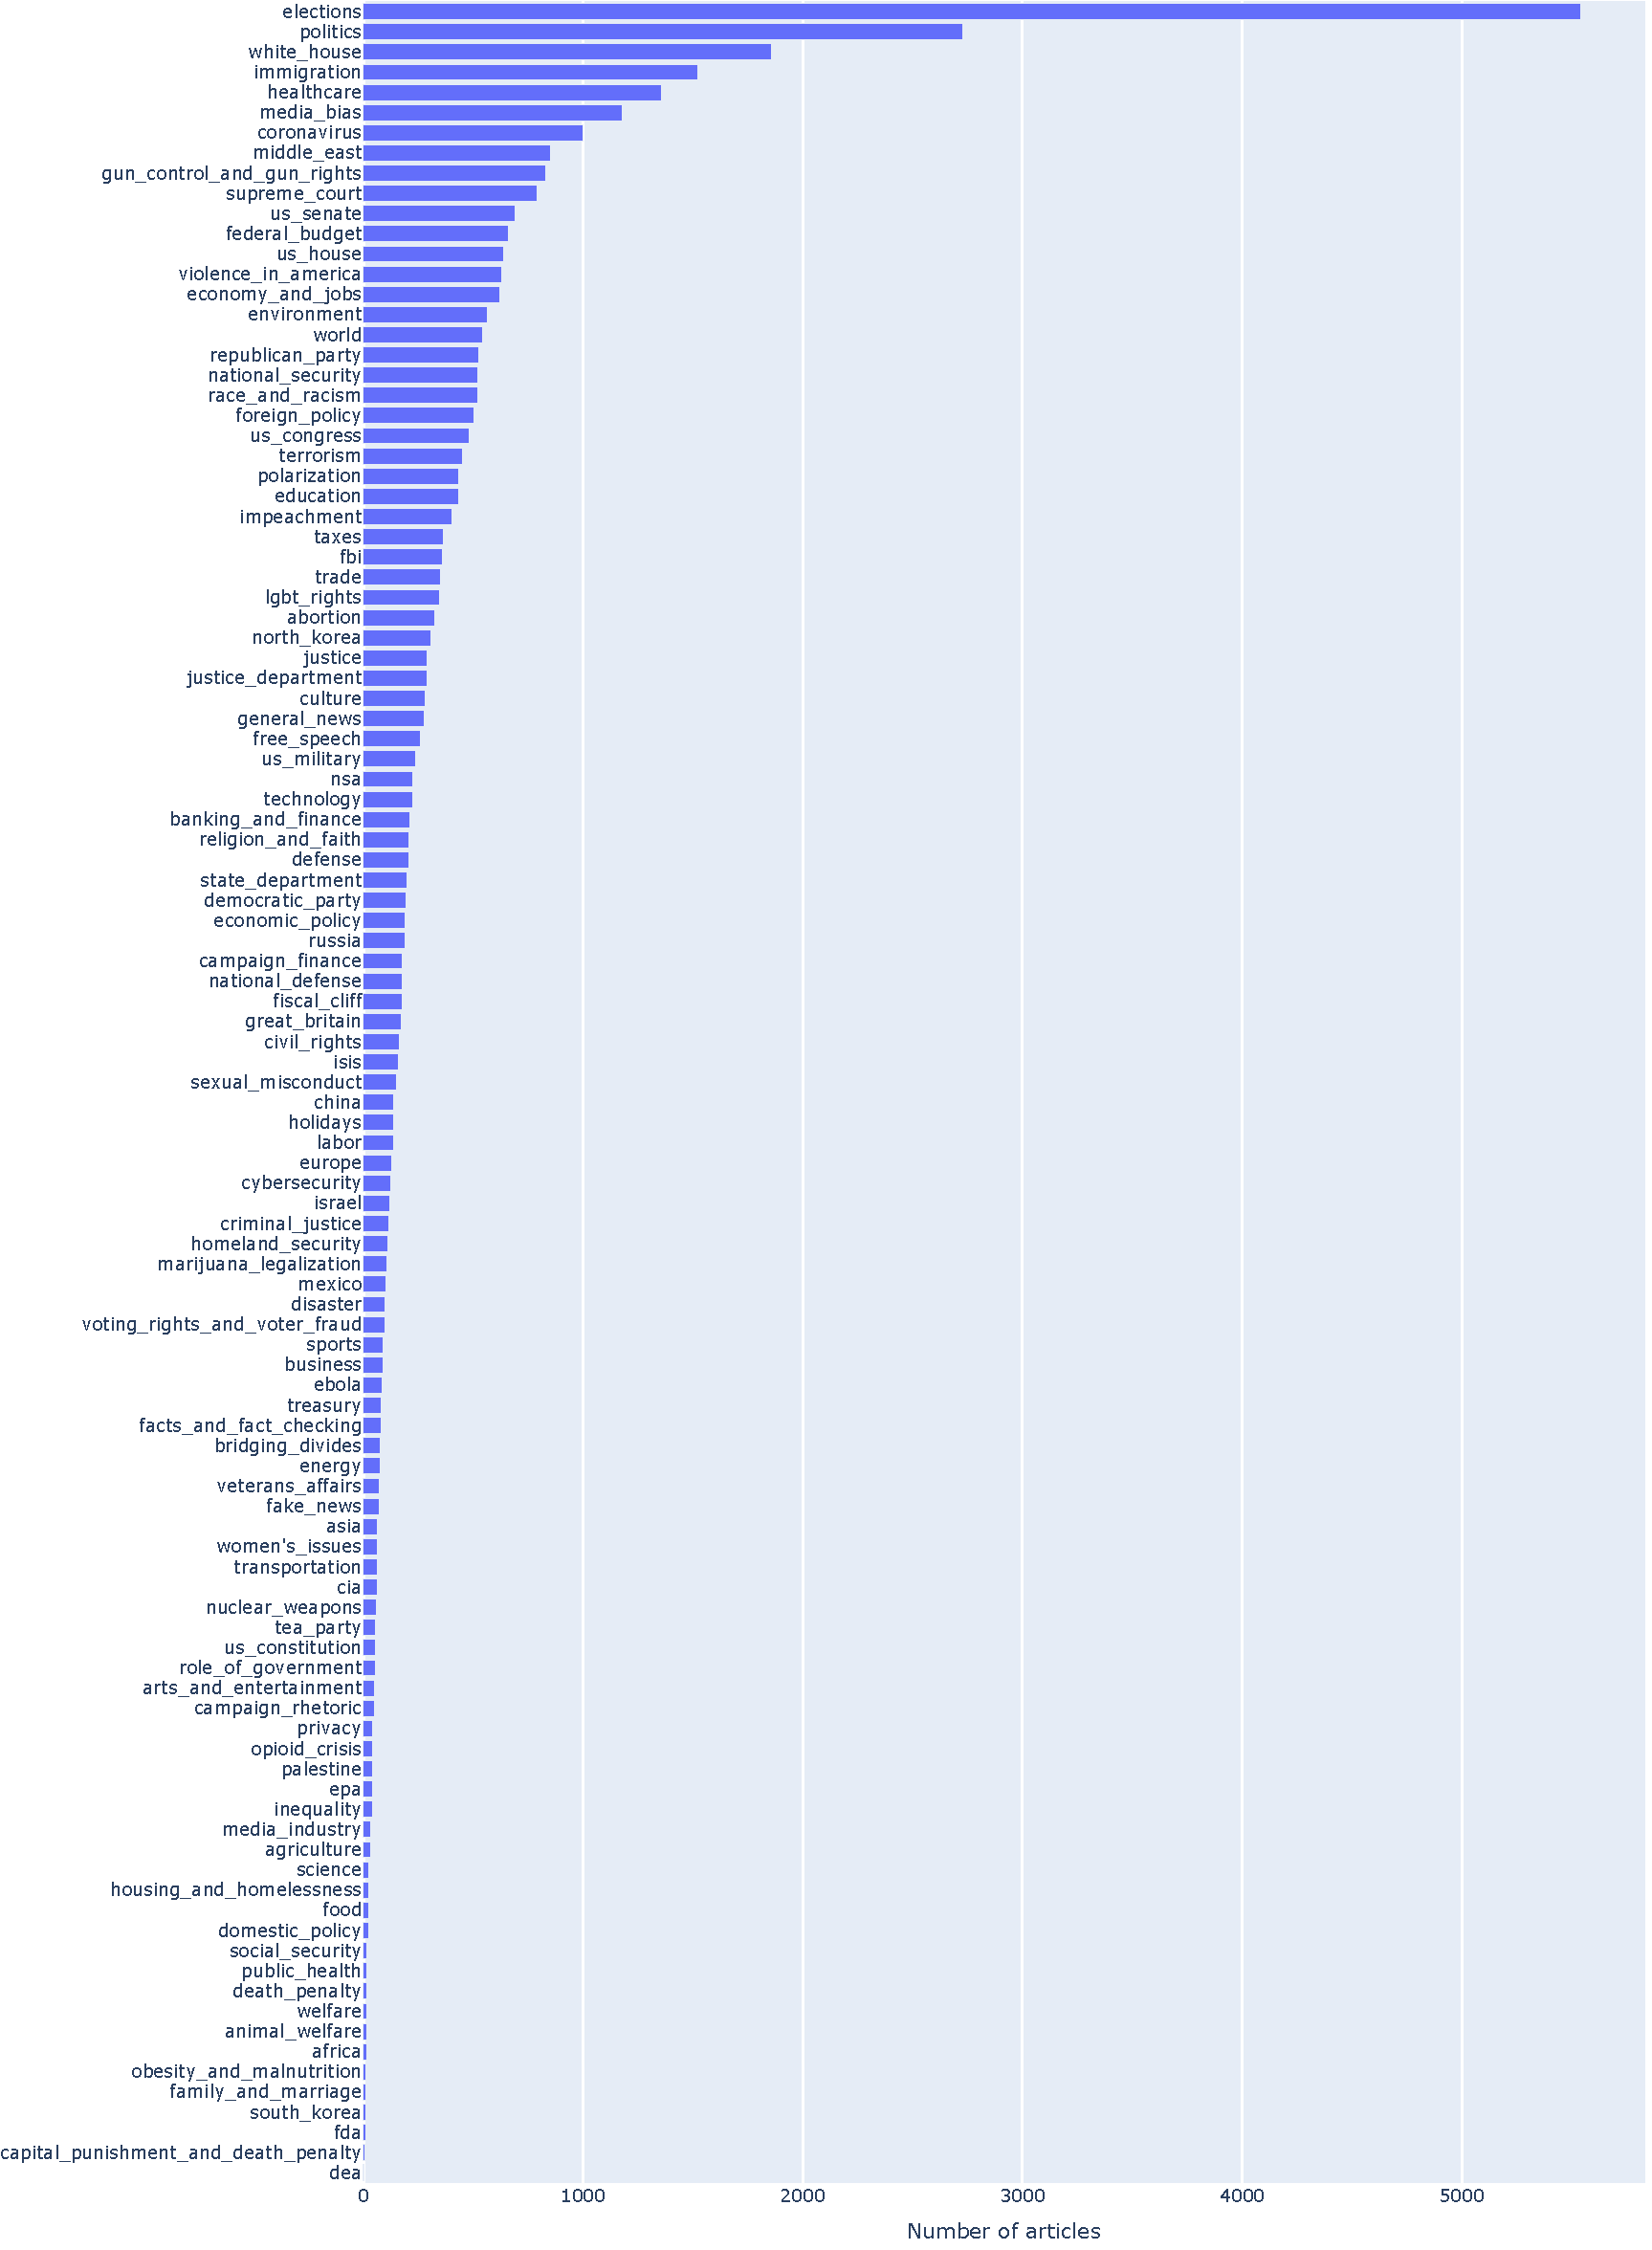
\includegraphics[width=\linewidth]{figures/baly_original_topics.pdf}
    \caption{Original topics of \texttt{Baly} dataset}
    \label{fig:baly_original_topics}
\end{figure}

These topic labels are given by the AllSides team with an unknown criteria, and the above shows how diverse and not-uniformed they are.


\subsubsection{Coarse Topics}

In this section we take into consideration the TextRazor coarseTopics annotations. TextRazor is a commercial API that allows to analyse topics, entities and to perform other NLP-related tasks (e.g. classify documents, …).
Regarding the topics, it provides coarseTopics, which are 17 very high-level topics (Belief, Business, Culture, Education, Health, Language, Law, Leisure, Mathematics, Nature, Politics, Science, Sports, Technology, Violence, Weather).
Each document is assigned with the top 5/6 matching coarseTopic, each one with a relevance score which ranges in [0,1]. Those scores don’t sum to 1. Each document is assigned to multiple topic, not a single one.

\paragraph{Most relevant topic Only}

Most relevant topic only
Each article only associated with the first (most important) topic. The topics from the second onwards are discarded.

\begin{figure}[!htbp]
    \centering
    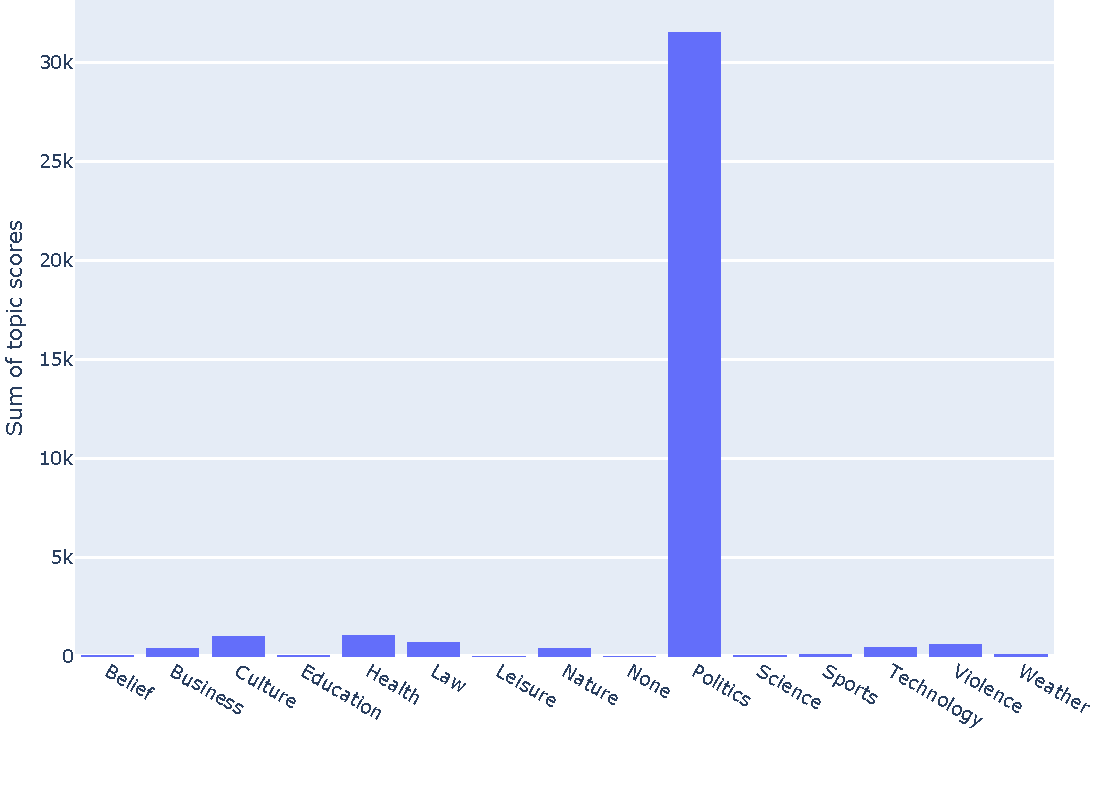
\includegraphics[width=\linewidth]{figures/baly_coarse_first.pdf}
    \caption{Coarse Topics most relevant of \texttt{Baly} dataset}
    \label{fig:baly_coarse_first}
\end{figure}

This shows that the dataset is highly unbalanced on Politics. This makes this topic annotation highly unusable.

\paragraph{Weighted (multi-topic)}
If we consider each of the 5/6 topic for each article and not only the first one, we get the following distribution:

\begin{figure}[!htbp]
    \centering
    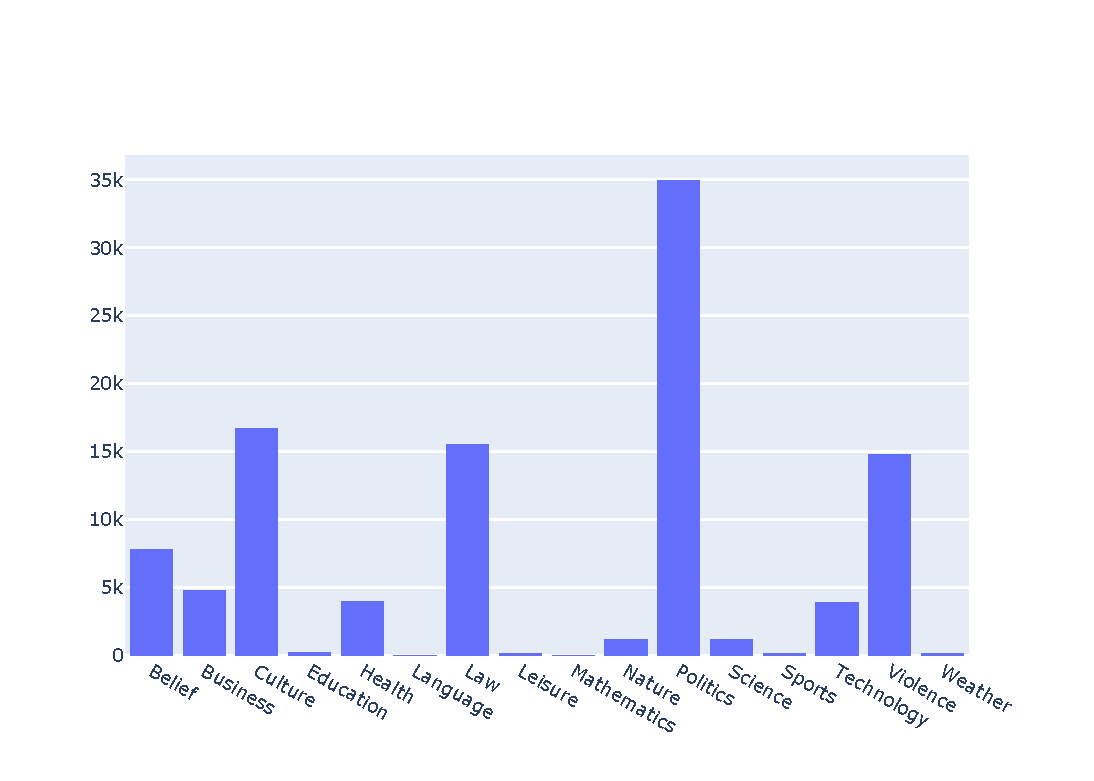
\includegraphics[width=\linewidth]{figures/baly_coarse_weighted.pdf}
    \caption{Coarse Topics weighted of \texttt{Baly} dataset}
    \label{fig:baly_coarse_weighted}
\end{figure}

We can see that the distribution is slightly unbalanced towards politics, then culture, law and violence. This looks like the topics are not too unbalanced, but we have to remember that we would like to have a single document to be categorised only with one topic, and this is not the case.

\subsubsection{Fine-Grained Topics}

\subsubsection{Derived from Entity types}

Freebase Taxonomy revised by TextRazor

entity propaganda feature computation
For each entity, compute the total/average propaganda techniques that co-occur in the same sentence %by each political leaning.
E.g.: “Donald Trump” used a lot of times with “Doubt” % from the Left leaning.

Interesting direction:
With Entity linking (provided by TextRazor) it is possible to find common attributes of the entities that make them targets of %Left/Right 
propaganda. E.g., a category of people as repeated target of Propaganda.


\subsubsection{IPTC Topics}

Expecially developed for news
Hierarchical


Problem: topic is very unbalanced on this dataset (everything about “politics”)
Breaking down with respect to topic, is not helpful to find differences between L/C/R if the topic splitting is very unbalanced and very generic.
When breaking a dataset of news articles we want to have the possibility to break down the topic enough to see differences. (e.g. In which topics the Left/Right are enough different in how they use propaganda?)



IPTC mediatopics
TextRazor gives in response 10 mediatopics for each article, each one with a score

\paragraph{Most relevant topic only}
All levels, only pick first one (most important)

TODO figure


Problem: only politics and government.
How to solve: when multiple labels are given, avoid the most broad/common ones. E.g.: politics:1.0, politics>elections: 0.85 → choose elections

What if, instead of trying dirty ways to select only one topic for each article, we keep the multi-topic annotations?
- Each article instead of having only one topic, is a distribution over a set of topics
- In the downstream tasks we can use this distribution as the topic description (why should it be only one topic?)
- If we proceed in this way, we should also do the same analysis with the standard topic distribution (not mediatopics)


\paragraph{Weighted full taxonomy}
Each article can belong to multiple categories.

\begin{figure}[!htbp]
    \centering
    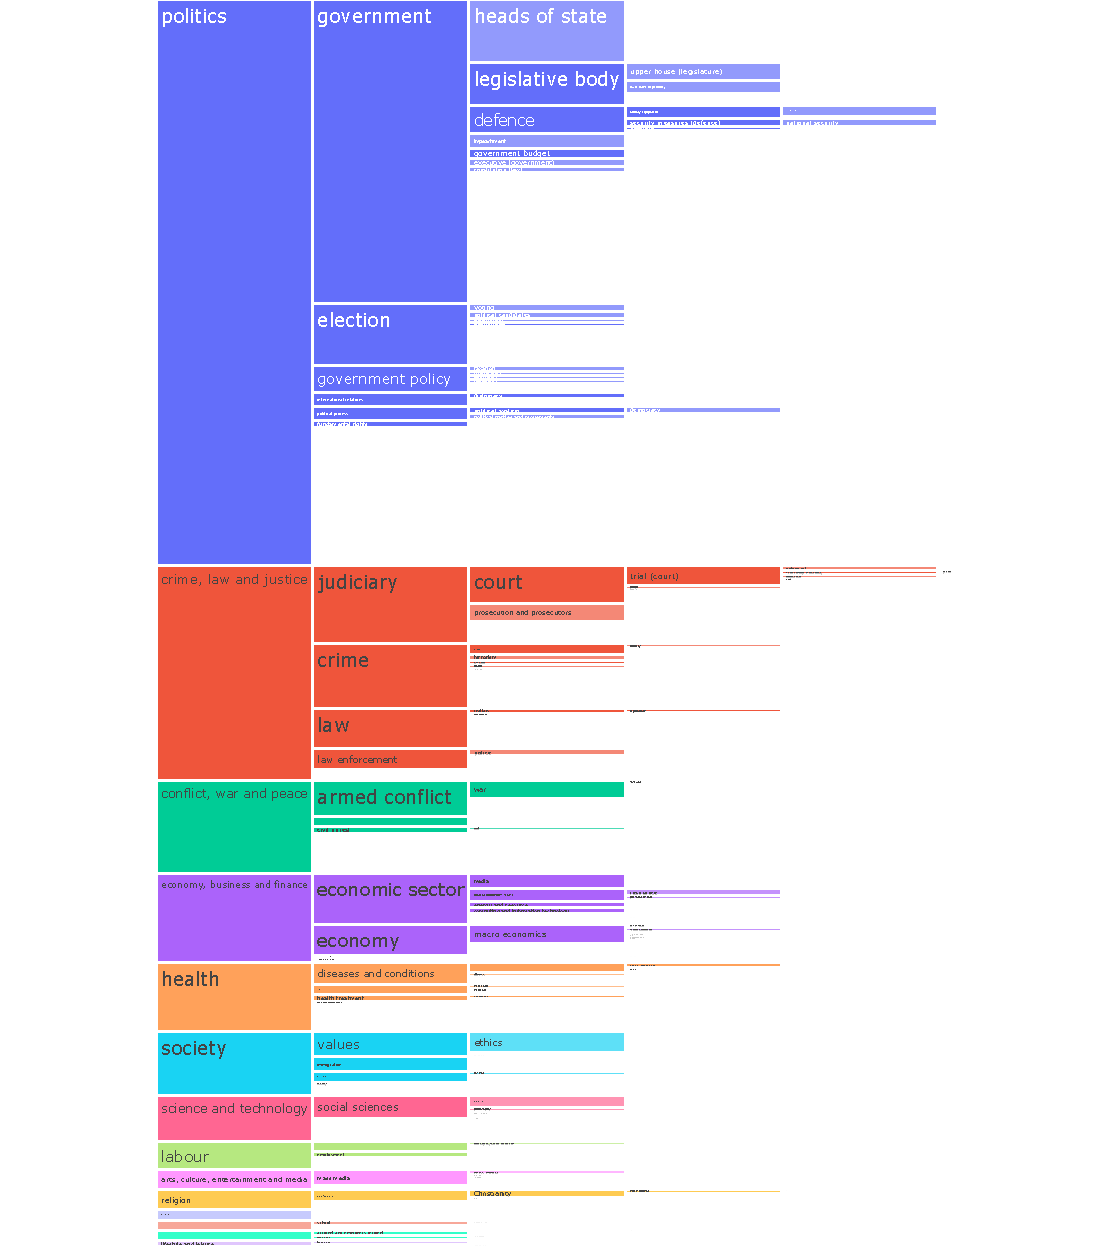
\includegraphics[width=\linewidth]{figures/baly_iptc_weighted.pdf}
    \caption{IPTC topics weighted of \texttt{Baly} dataset}
    \label{fig:baly_iptc_weighted}
\end{figure}


Options:
Multi-topic weighted complex solution
Only see what happens in specific topic with the classifier
Input topics as features and see classifier what produces:
Need to encode the topics hierarchically
Need model (neural network) on top that can combine the features. Single-layer neural network cannot, need 2 layers at least



\section{Topic and Propaganda and Leaning}

TODO introduce combined

\subsection{Breakdown of propaganda by topics}

This section contains analysis of how propaganda is distributed across topics and what differences topics contain in terms of propaganda.
Assumption: propaganda is used for certain topics in a very recognisable way to push for the ideas of the leaning of the source

RQ1: \emph{How propaganda changes across topics and leanings?}

Experiment 4.3: 
- topic breakdown: AllSides Topics, IPTC
- shapes of propaganda/sentiment


Types of shapes (propaganda)
(look at purple: propaganda)

Blue is sentiment (+ and -) and purple is propaganda. 
y axis in the fraction of terms marked as sentiment/propaganda.

\subsubsection{Custom Topics (AllSides)}

\subsubsection{Coarse Topics}

\subsubsection{Fine-Grained Topics}

\subsubsection{Derived from Entity Types}

entity propaganda feature computation
For each entity, compute the total/average propaganda techniques that co-occur in the same sentence by each political leaning. E.g.: “Donald Trump” used a lot of times with “Doubt” from the Left leaning.

Interesting direction:
With Entity linking (provided by TextRazor) it is possible to find common attributes of the entities that make them targets of Left/Right propaganda. E.g., a category of people as repeated target of Propaganda.

\subsubsection{IPTC Topics}

\paragraph{Correlation Left vs Right}
Exploratory way: observe the correlation between features of the left and features of the right. If correlation is high, it means that the differences are small. Instead if the correlation is low, it means that there exist differences between left and right.


Correlation between L/R of Propaganda quantities (18 values for each article) across topics
The hope is to see that in some subtopics the correlation is low, meaning that the propaganda quantities differ significantly between Left and Right for the subtopic.
On the full dataset, this propaganda feature was not very useful, so let’s see what happens in all the subtopics.

TODO figure

Scale: blue=correlation high, red=correlation low, grey=not computable (all 0)

This is clearly a negative result. This means that the propaganda quantities are not useful at all. Let’s check what happens with other features:



\subsection{Predicting Leaning from topics and propaganda}

In this section we aim to analyse the relationship between topics, propaganda and leaning from a different perspective.

RQ2: \emph{knowing the topic, does it make classification (prop-->leaning) easier?}

7: topics+propaganda for political leaning prediction


\section{Discussions}

What is the conclusion of this work?